% This file is part of the StegX project.
% Copyright (C) 2018  StegX Team
% 
% StegX is free software: you can redistribute it and/or modify
% it under the terms of the GNU General Public License as published by
% the Free Software Foundation, either version 3 of the License, or
% (at your option) any later version.
% 
% This program is distributed in the hope that it will be useful,
% but WITHOUT ANY WARRANTY; without even the implied warranty of
% MERCHANTABILITY or FITNESS FOR A PARTICULAR PURPOSE.  See the
% GNU General Public License for more details.
% 
% You should have received a copy of the GNU General Public License
% along with this program.  If not, see <https://www.gnu.org/licenses/>.

\documentclass[11pt]{article}
%\documentclass{book}
\usepackage[utf8]{inputenc}
\usepackage[T1]{fontenc}
\usepackage[french]{babel}
\usepackage[top=1.8cm, bottom=1.8cm, left=1.8cm, right=1.8cm]{geometry}
\usepackage[linktocpage,colorlinks=false]{hyperref}
\usepackage{graphicx}
\usepackage{epsfig}
\usepackage{amssymb}
\usepackage{amsmath}
\usepackage{array}
\usepackage{subfig}
\usepackage{multicol}
\usepackage{caption}
\usepackage{listings}
\usepackage{algorithm}
\usepackage{algorithmic}
\hypersetup{
    colorlinks=true,
    breaklinks=true,
    urlcolor=red,
}
\parskip=5pt

\title{\huge{\textbf Manuel d'utilisation}}
\author{AYOUB Pierre, BASKEVITCH Claire, BESSAC Tristan, \\
CAUMES Clément, DELAUNAY Damien, DOUDOUH Yassin}
\date{Mercredi 25 Mai 2018}

\begin{document}

\maketitle
\vspace{20em}
\begin{center}
\includegraphics{pictures/Application.png}\end{center}
\newpage

\tableofcontents

\newpage

\section{Installation et désinstallation}

\subsection{Installation sous Linux}

\underline{Installation standard sous un Debian-like :}

\begin{itemize}
\item Installer l'application en utilisant une interface à APT (par exemple en
    double cliquant dessus), ou en utilisant la commande `sudo apt-get install
    ./StegX-xxx.deb` depuis le répertoire ou ce situe l'installateur.
\end{itemize}

\underline{Installation depuis les sources :}

\begin{itemize}
\item Télécharger le compilateur GCC, GTK+-3.0 et CMake (dernière version). Dans
    le dossier racine du projet, exécuter les commandes suivantes :
\item mkdir build 
\item cd build
\item cmake ..
\end{itemize}

\hspace{1cm}
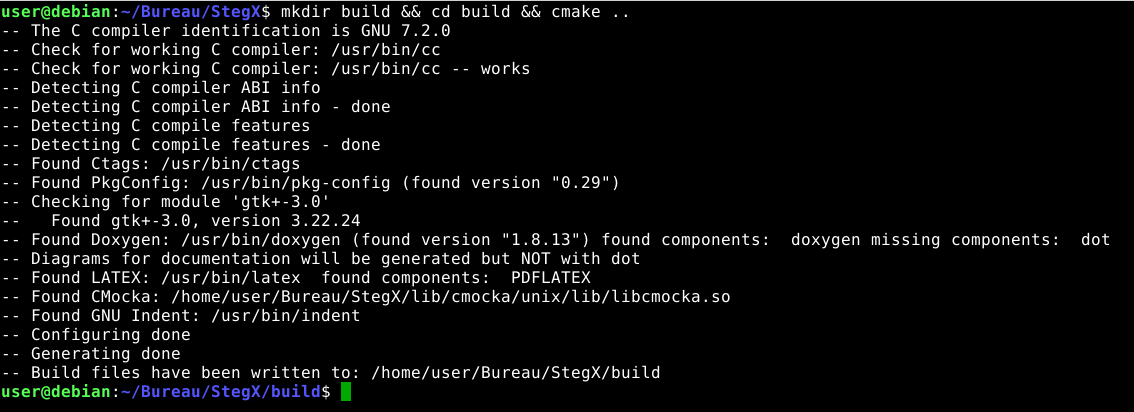
\includegraphics[scale=0.5]{pictures/build.png}
\vspace{0.5cm}

\begin{itemize}
\newpage
\item make
\end{itemize}

\hspace{2cm}
\vspace{0.5cm}
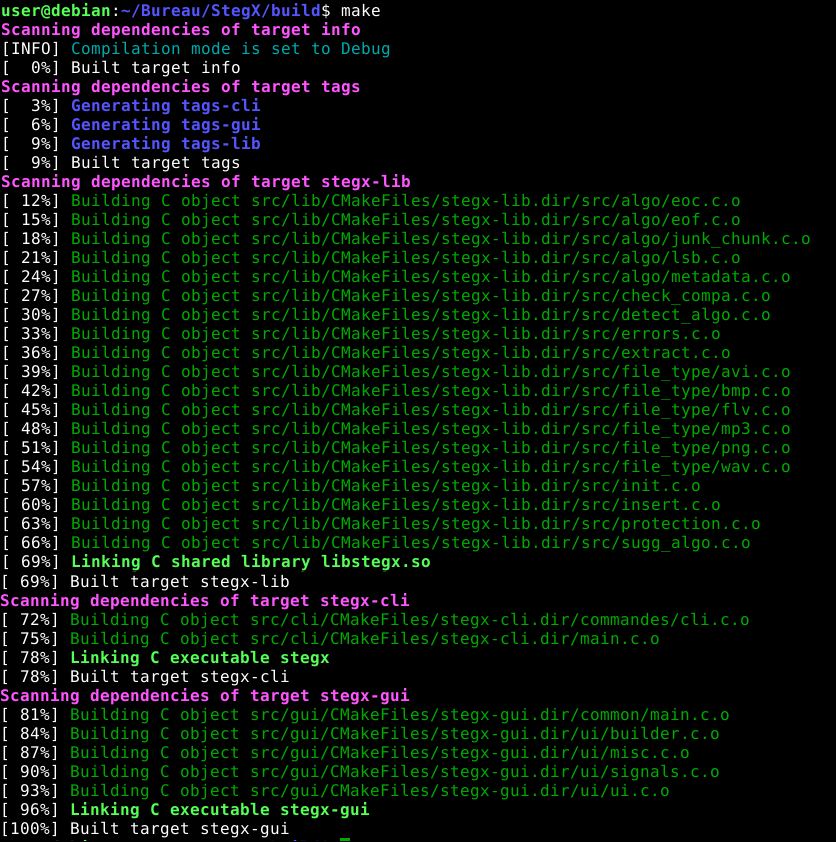
\includegraphics[scale=0.5]{pictures/make.png}


\begin{itemize}
\item sudo make install
\end{itemize}

\hspace{1cm}
\vspace{0.5cm}
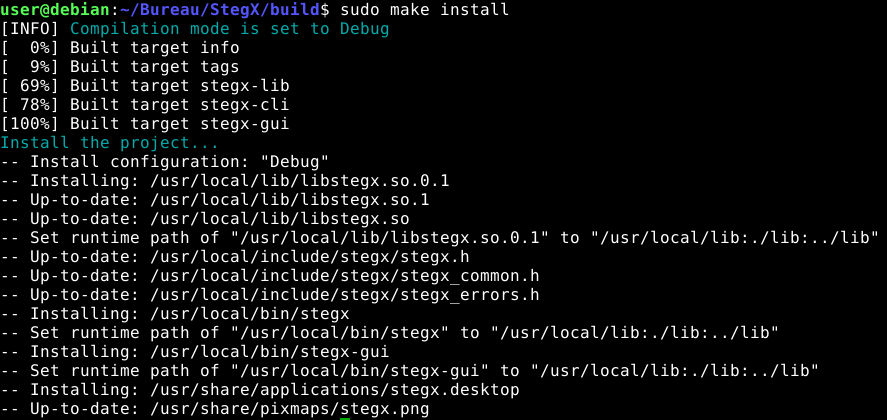
\includegraphics[scale=0.5]{pictures/install.png}

\subsection{Désinstallation sous Linux}

Pour désinstaller StegX, taper dans sur le terminal : \newline
\underline{Après une installation standard sous un Debian-like :}
\begin{itemize}
\item sudo apt remove stegx
\end{itemize}
\underline{Après une installation depuis les sources :}
\begin{itemize}
\item sudo make uninstall
\end{itemize}

\subsection{Installation sous Windows}

\begin{itemize}
\item Double cliquer sur StegX-x.x.x-win64.exe afin de lancer l'installateur.
\end{itemize}

\hspace{1cm}
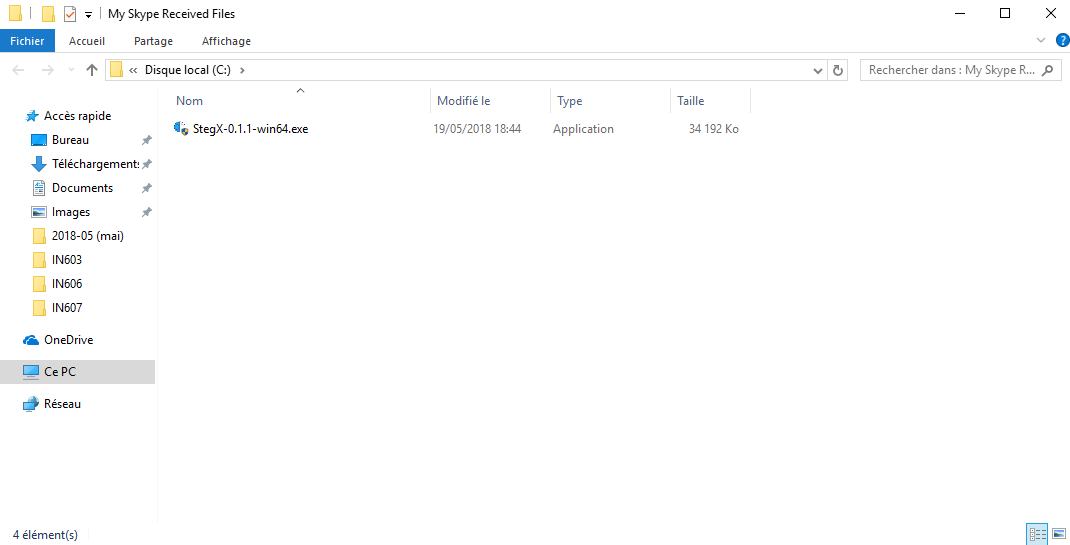
\includegraphics[scale=0.5]{pictures/ouverture.png}
\vspace{1cm}

\begin{itemize}
\item Cliquer sur "Suivant". 
\end{itemize}

\hspace{1cm}
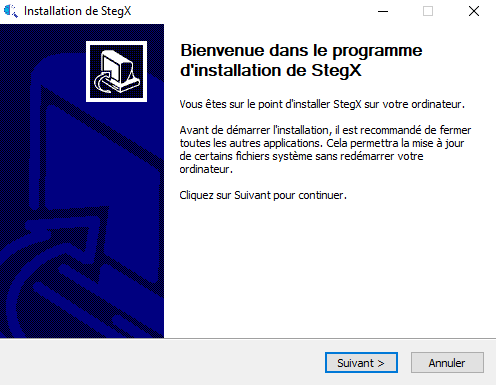
\includegraphics[scale=1]{pictures/presentation.png}
\vspace{1cm}
\newpage
\begin{itemize}
\item Cliquer sur "J'accepte" après avoir pris connaissance de la licence. 
\end{itemize}

\hspace{1cm}
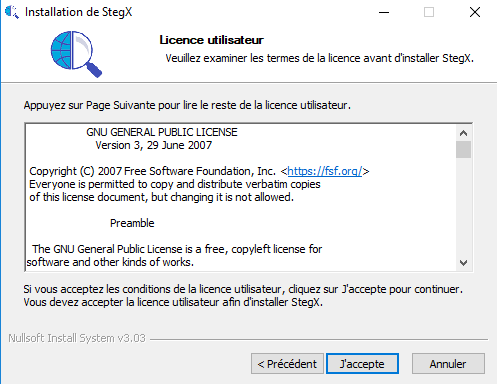
\includegraphics[scale=1]{pictures/licence.png}
\vspace{1cm}

\begin{itemize}
\item Cliquer sur "Suivant". 
\end{itemize}

\hspace{1cm}
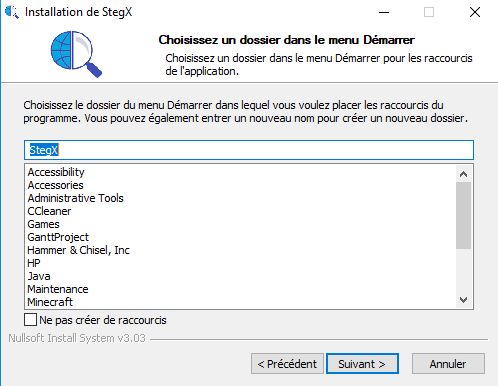
\includegraphics[scale=1]{pictures/debut.png}
\vspace{1cm}

\begin{itemize}
\item Sélectionner le deuxième ou le troisième choix si vous voulez pouvoir
    lancer l'interface en ligne de commande en tapant "stegx" dans
    l'interpréteur de commande de Windows. Sinon, sélectionner le premier
    choix. Cliquer sur "Suivant". 
\end{itemize}

\hspace{1cm}
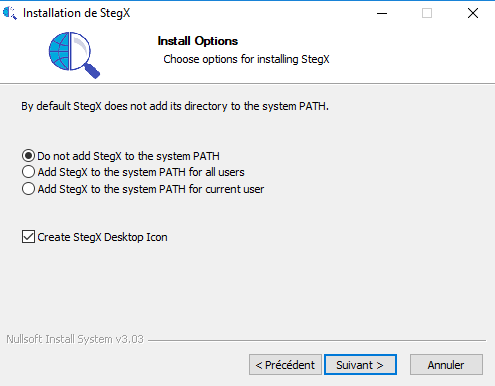
\includegraphics[scale=1]{pictures/path.png}
\vspace{1cm}

\begin{itemize}
\item Cliquer sur "Suivant". 
\end{itemize}

\hspace{1cm}
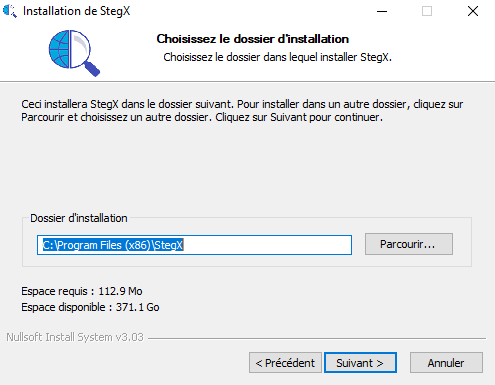
\includegraphics[scale=1]{pictures/taille.png}
\vspace{1cm}

\begin{itemize}
\item Choisir les composants de l'application à installer (interface 
en ligne de commande et/ou interface graphique). 
\item Cliquer sur "Suivant". 
\end{itemize}

\hspace{1cm}
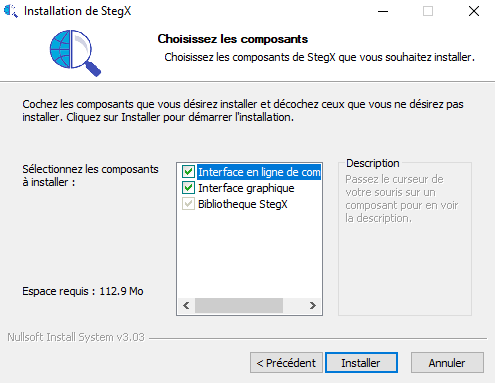
\includegraphics[scale=1]{pictures/choix.png}
\vspace{1cm}

\begin{itemize}
\item Attendre la fin de l'installation.
\item Cliquer sur "Suivant". 
\end{itemize}

\hspace{2.5cm}
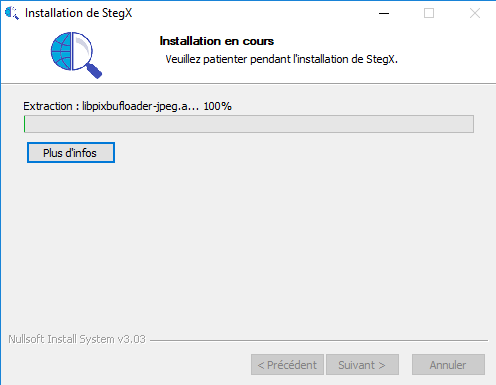
\includegraphics[scale=0.8]{pictures/installation.png}
\vspace{1cm}
\newpage

\begin{itemize}
\item Cliquer sur "Fermer". 
\end{itemize}

\hspace{1cm}
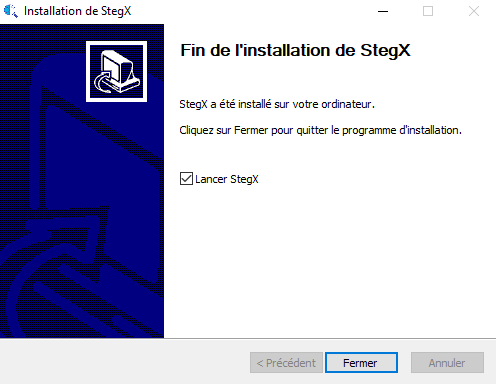
\includegraphics[scale=1]{pictures/fin.png}
\vspace{1cm}

\subsection{Désinstallation sous Windows}

\begin{itemize}
\item Accéder au panneau de configuration, cliquer sur désinstaller un programme,
sélectionner StegX et cliquer sur désinstaller.
\end{itemize}

\hspace{3cm}
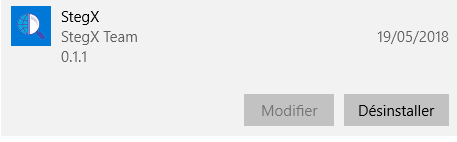
\includegraphics[scale=0.6]{pictures/desinstall.png}
\newpage

\section{Manuel du développeur}

\subsection{Réalisation des tests unitaires}

Pour réaliser les tests unitaires présents dans le dossier "StegX/test/lib/" : 
\begin{itemize}
\item Aller dans le dossier "build/".
\item Taper sur le terminal "make check". Les fichiers créés seront créés 
dans le dossier "build/".
\end{itemize}
\vspace{0.5cm}
\hspace{3cm}
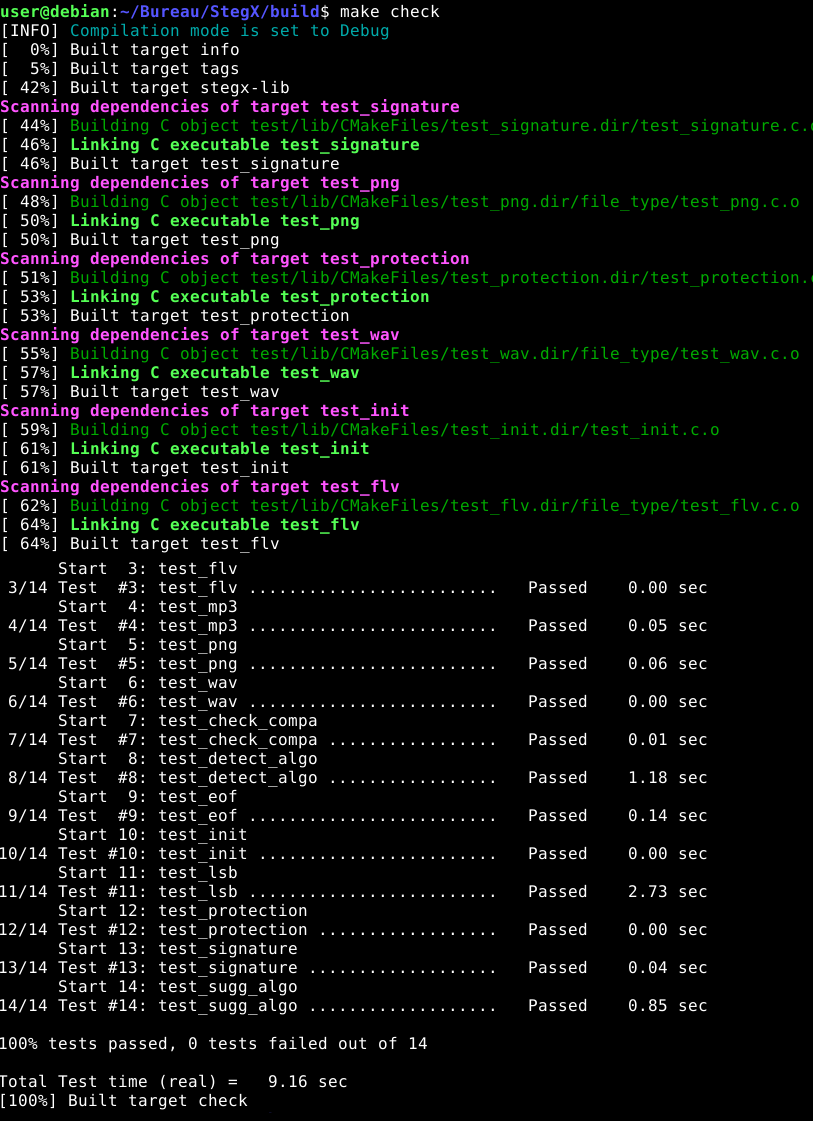
\includegraphics[scale=0.45]{pictures/check.png}
\vspace{1cm}

\subsection{Génération de la documentation}
\begin{itemize}
\item Aller dans le dossier "build/".
\item Taper sur le terminal "make doc". Les fichiers créés seront créés 
dans le dossier "build/". 
\end{itemize}
\vspace{0.5cm}
\hspace{3cm}
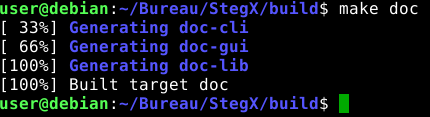
\includegraphics[scale=0.7]{pictures/doc.png}


\section{Manuel de l'utilisateur}

\subsection{Utilisation de l'interface en ligne de commande}

Pour voir la présentation de l'application en ligne de commande :
\begin{itemize}
\item Taper sur le terminal "stegx -a".
\end{itemize}

\vspace{0.5cm}
\hspace{0.5cm}
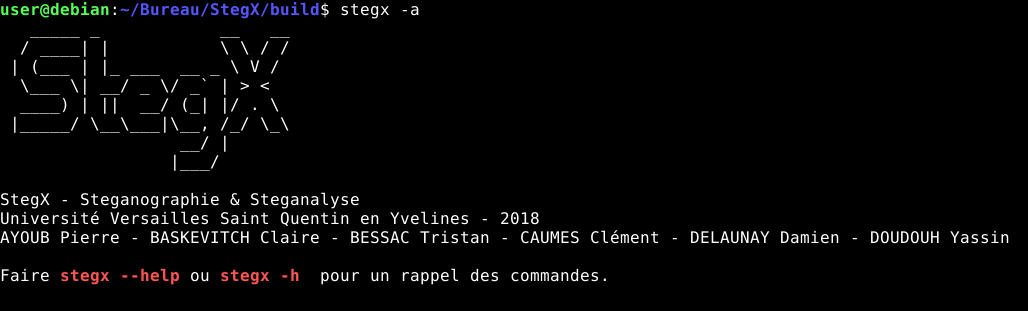
\includegraphics[scale=0.6]{pictures/present.png}
\vspace{1cm}

Pour visualiser les différentes commandes : 
\begin{itemize}
\item Taper sur le terminal "stegx -h".
\end{itemize}

\vspace{0.5cm}
\hspace{-0.5cm}
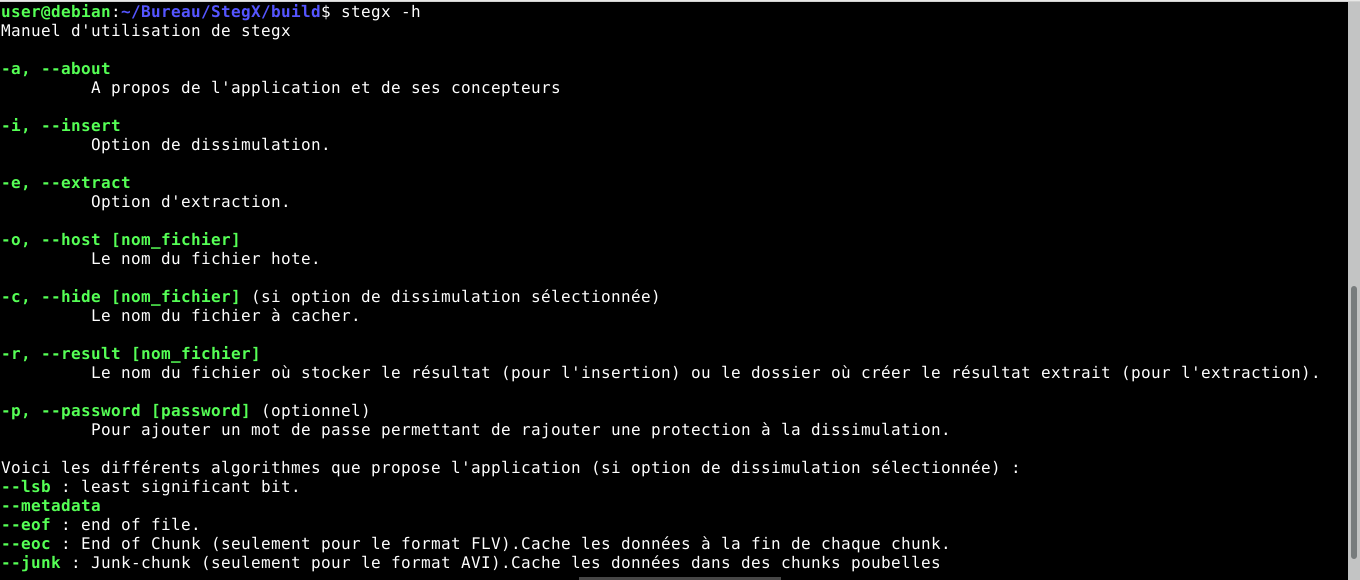
\includegraphics[scale=0.5]{pictures/help.png}
%\vspace{1cm}

\subsubsection{Insertion}

Pour réaliser une insertion, voici un exemple réalisé sur de vrais 
fichiers : 

\vspace{0.5cm}
\hspace{-2cm}
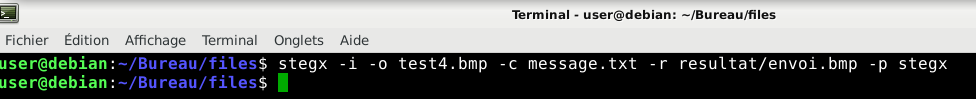
\includegraphics[scale=0.8]{pictures/insertion.png}
\vspace{1cm}

\subsubsection{Extraction}

Pour réaliser une extraction, voici un exemple réalisé sur de vrais 
fichiers :

\vspace{0.5cm}
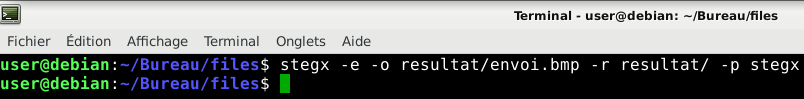
\includegraphics[scale=0.8]{pictures/extraction.png}

\subsection{Utilisation de l'interface graphique}

Pour utiliser l'application avec l'interface graphique, taper sur le 
terminal "stegx-gui" ou cliquer sur l'icône de StegX dans les raccourcis 
logiciels. 

Pour visualiser la présentation de l'application, cliquer sur "A propos". 

\vspace{0.5cm}
\hspace{2cm}
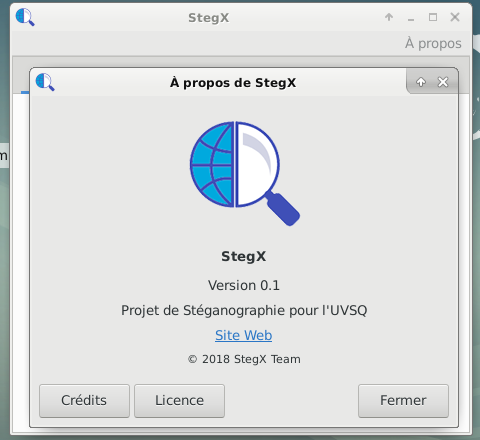
\includegraphics[scale=0.8]{pictures/a_propos.png}
\vspace{1cm}

\subsubsection{Insertion}

Pour faire une dissimulation d'un fichier à cacher dans un fichier hôte : 
\begin{itemize}
\item Cliquer sur "Dissimulation".
\item Choisir un fichier hôte. 
\item Choisir un fichier à cacher. 
\item Choisir l'emplacement du fichier à créer. 
\item Choisir un nom pour le fichier à créer. 
\item Choisir un mot de passe [facultatif]. 
\item Cliquer sur "Analyser". 
\end{itemize}

\vspace{0.5cm}
\hspace{-2cm}
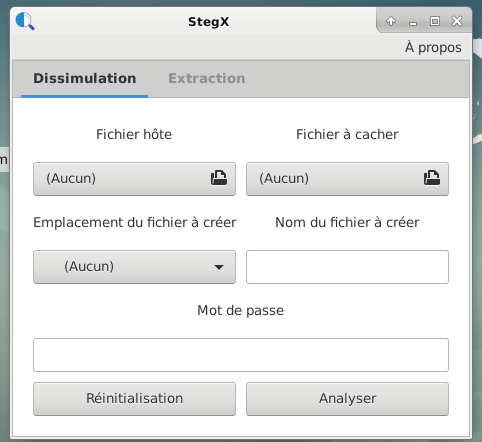
\includegraphics[scale=0.8]{pictures/ouverture2.png}
\vspace{1cm}
\hspace{0.2cm}
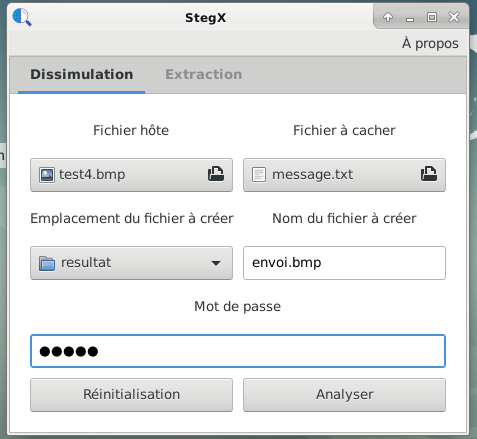
\includegraphics[scale=0.8]{pictures/insertion_1.png}

L'analyse du fichier hôte et du fichier à cacher est terminée: 
\begin{itemize}
\item Cliquer sur "Valider". 
\end{itemize}

\vspace{0.5cm}
\hspace{2cm}
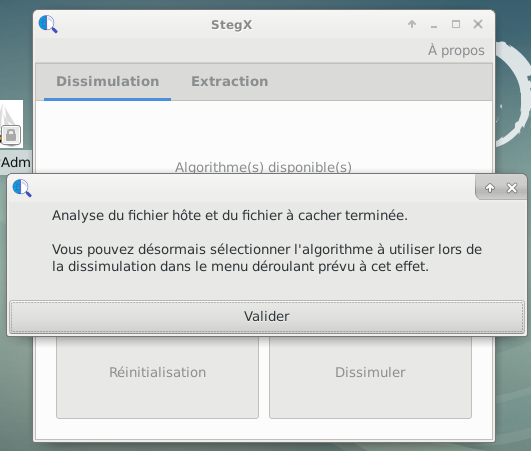
\includegraphics[scale=0.8]{pictures/insertion_2.png}
\vspace{1cm}

Un ou plusieurs algorithmes est proposé : 
\begin{itemize}
\item Choisir l'algorithme à utiliser pour la dissimulation.
\item Cliquer sur "Dissimuler". 
\end{itemize}

\vspace{0.5cm}
\hspace{2cm}
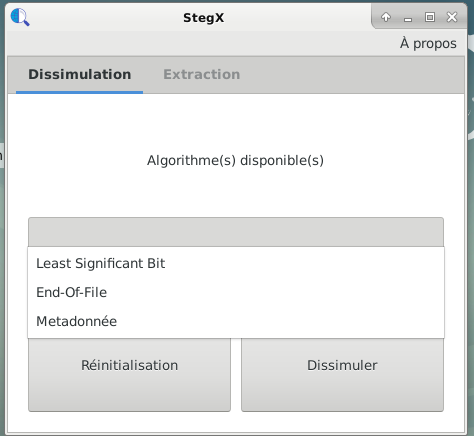
\includegraphics[scale=0.8]{pictures/insertion_3.png}


\subsubsection{Extraction}

Pour réaliser une extraction d'un fichier caché dans un fichier à analyser : 
\begin{itemize}
\item Cliquer sur "Extraction".
\item Choisir un fichier hôte (fichier à analyser). 
\item Choisir l'emplacement du fichier extrait. 
\item Choisir un mot de passe [facultatif]. 
\item Cliquer sur "Extraire". 
\end{itemize}

\vspace{1cm}
\hspace{-2cm}
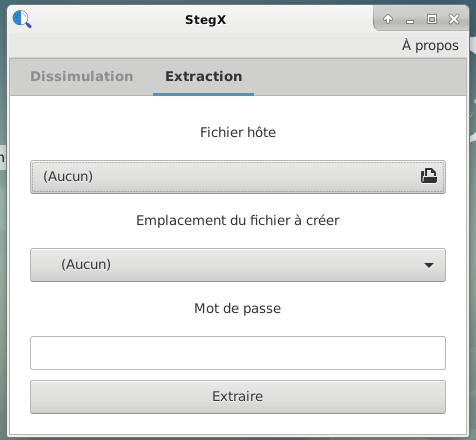
\includegraphics[scale=0.8]{pictures/extraction_1.png}
\vspace{1cm}
\hspace{0.2cm}
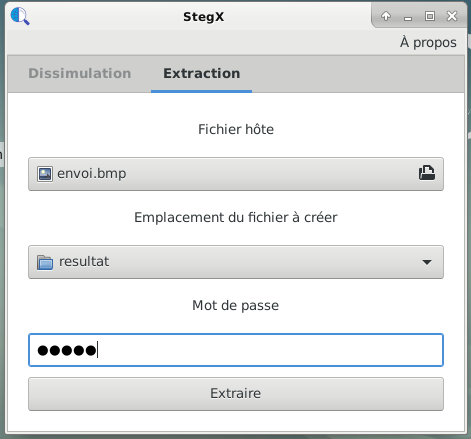
\includegraphics[scale=0.8]{pictures/extraction_2.png}

Lorsque l'extraction est terminée, une fenêtre s'ouvre : 

\hspace{2.5cm}
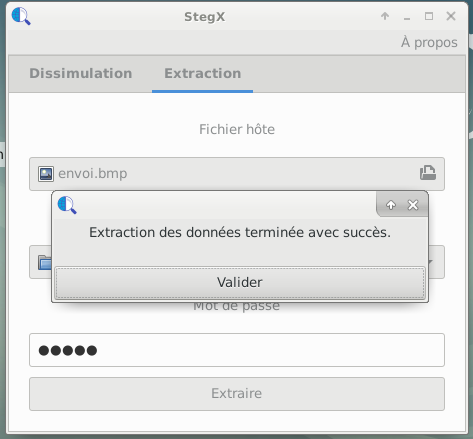
\includegraphics[scale=0.8]{pictures/extraction_3.png}
\vspace{1cm}

\end{document}
